% !TEX program = pdflatex
% Supplementary Appendix for the ECAI submission (separate PDF).
% Compiled with the same local ECAI-geometry stand-in. Not page-limited.
\documentclass{ecai}
\pdfsuppressptexinfo=-1
\usepackage[numbers,sort&compress]{natbib}
\usepackage{times}
\usepackage[T1]{fontenc}
\usepackage[utf8]{inputenc}
\usepackage{microtype}
\usepackage{graphicx}
\usepackage{booktabs}
\usepackage{amsmath}
\usepackage{amssymb}

\title{Supplementary Appendix:\\
Status Fidelity Under Chained Memory Rewriting}

\author{Anonymous ECAI submission}

\newcommand{\st}[1]{\textsc{#1}}

\begin{document}
\maketitle
\onecolumn
\appendix

\noindent This appendix accompanies the main paper and is not part of the
page-limited submission. Section letters match the in-text pointers
(Supplementary Appendix~A--F), followed by prompt sources, annotation and
reliability details, and scenario examples.

\section{Status Tuple and Conditions}
\label{app:tuple}

\begin{table}[h]
\centering
\small
\begin{tabular}{p{0.22\textwidth}p{0.66\textwidth}}
\toprule
Component & Values / definition \\
\midrule
Epistemic & UNKNOWN, POSSIBLE, PROBABLE, SUPPORTED, ESTABLISHED, REJECTED \\
Intentional & NOT\_EXPRESSED, CONSIDERING, INTERESTED, INTENDING, COMMITTED, EXECUTING, COMPLETED, CANCELLED, NOT\_INTENDED \\
Conditional & condition state UNKNOWN, ACTIVE\_UNSATISFIED, SATISFIED, FAILED, WAIVED; action state stored separately \\
Polarity & affirmative, negated \\
Scope & proposition object and its qualifiers \\
Time & evaluation time $t$; latest supported state up to $t$ \\
\bottomrule
\end{tabular}
\caption{Status tuple components. Confirmatory annotation uses collapsed label
sets (Section~3 of the main paper).}
\label{tab:tuple}
\end{table}

\begin{table}[h]
\centering
\small
\begin{tabular}{p{0.20\textwidth}p{0.68\textwidth}}
\toprule
Condition & Control it provides \\
\midrule
Raw & no compression reference \\
Direct & one writer call, final budget \\
Recursive & shrinking intermediate budgets \\
Rewrite-matched & constant intermediate budgets, same call count as recursive \\
Repeated-direct & same writer-call count, no shrinking \\
Source-peek & original dialogue visible at every rewrite \\
Paraphrase & prompt variation \\
Temperature 1/2 & sampling variation \\
Path schedule 2 & alternative rewrite schedule \\
Retrieval & source access at query time \\
\bottomrule
\end{tabular}
\caption{Transformation conditions in Study 1.}
\label{tab:conditions}
\end{table}

\section{Study 2a Counts}
\label{app:synthetic}

\begin{table}[h]
\centering
\small
\begin{tabular}{lccccc}
\toprule
Variant & PROCEED & CONFIRM & ABSTAIN & Unauthorized & Evidence-consistent \\
\midrule
Present & 12 & 18 & 0 & 2/30 & 28/30 \\
Omitted & 0 & 30 & 0 & 0/30 & 20/30 \\
Distorted & 20 & 10 & 0 & 20/30 & 0/30 \\
No memory & 0 & 13 & 17 & 0/30 & 20/30 \\
\bottomrule
\end{tabular}
\caption{Study 2a decisions (30 trajectories; primary agent).}
\label{tab:synthetic}
\end{table}

\section{Bank Validation and Control Gates}
\label{app:bank}

The original 40 scenarios were rated by two humans on 1--5 scales (realism
4.113 pooled; status clarity 4.975; rule clarity 4.950; distortion plausibility
4.250; stake severity 3.350). \emph{Only-status-differs} was 38/40 yes-both
($\kappa$ 0.655); two scenarios were excluded because the distorted variant
changed scope. Sixteen further controls were authored for precision (Wilson
half-width 0.29--0.35 at $n=4$ versus 0.14--0.20 at $n=20$) and were validated
the same way after the main run (realism 4.969 pooled; status clarity 5.000;
rule clarity 4.969; distortion plausibility 4.312; stake severity 2.875;
\emph{only-status-differs} 15/16, $\kappa$ 1.000). Two thresholds are on
record: the protocol pre-specified $\ge 0.95$, and the validation sheet used
for these 16 controls accepted $\ge 0.90$. At 15/16 ($0.9375$) the expansion
set passes the looser threshold and fails the protocol one, so the expansion
gate is labeled a post-hoc decision. HEA-11 is the single failure: both
annotators said its distorted variant introduces a new proposition (the
doctor's stop order) rather than flipping the user's status. It is excluded
from the strict primary analysis and retained in an inclusive sensitivity, and
both denominators are reported.

\begin{table}[h]
\centering
\small
\begin{tabular}{lcccc}
\toprule
Variant & \multicolumn{2}{c}{Neutral} & \multicolumn{2}{c}{Action} \\
\cmidrule(lr){2-3}\cmidrule(lr){4-5}
 & EXEC & under & EXEC & under \\
\midrule
Present & 19/19 & 0 & 17/19 & 2/19 \\
Omitted & 7/19 & 12/19 & 2/19 & 17/19 \\
Distorted & 1/19 & 18/19 & 0/19 & 19/19 \\
No memory & 0/19 & 19/19 & 0/19 & 19/19 \\
\bottomrule
\end{tabular}
\caption{Authorized-execution controls: EXECUTE and under-action counts
(primary agent, strict 19-control set). The inclusive 20-control set, which
retains HEA-11, gives present 20/20 and 18/20, omitted 7/20 and 2/20, distorted
1/20 and 0/20, and no memory 0/20 in both forms.}
\label{tab:controls}
\end{table}

Item validity, mechanical output compliance, and semantic compliance are
reported separately. Present-status EXECUTE by model and form, strict 19
(inclusive 20): gemma3:12b 19/19 neutral and 17/19 action (20/20, 18/20);
qwen2.5:7b 15/19 and 9/19 (16/20, 10/20); mistral:7b 17/19 and 8/19 (18/20,
9/20); the gateway-reported model 19/19 in both forms (20/20). Mechanical
compliance is identical except for the gateway neutral cell, where AUT-11's
output begins with \texttt{EXECUTE} but omits the \texttt{DECISION:} prefix:
it is a mechanical parse failure (18/19) and a semantic EXECUTE (19/19).
Qwen's action form is exactly 10/20, which triggers the post-hoc half-floor
diagnostic (rate $\le 0.50$); the frozen protocol gate is only ``not at
floor'' (rate $> 0$), so 10/20 is reported as a boundary result rather than a
preregistered failure.

\begin{table}[h]
\centering
\small
\begin{tabular}{lc}
\toprule
Code & Count \\
\midrule
D1 followed distorted memory & 34 \\
O2 mention as commitment & 5 \\
O1 asserted unstated commitment & 0 \\
O3 request as authorization & 0 \\
\bottomrule
\end{tabular}
\caption{Unauthorized-reason codes for all 39 over-commitment executions of the
primary agent (post hoc, analyst, gold-unblinded). The gateway model's 65
executions split identically: 54 D1, 11 O2, 0 O1/O3.}
\label{tab:reasons}
\end{table}

\section{Second-Writer Replication}
\label{app:repl}

\begin{table}[h]
\centering
\small
\begin{tabular}{lcccc}
\toprule
Condition & Faithful & Omission & Unsupported & Ambiguous \\
\midrule
Direct & 11/12 & 1/12 & 0/12 & 0/12 \\
Repeated-direct & 11/12 & 1/12 & 0/12 & 0/12 \\
Source access & 10/12 & 1/12 & 1/12 & 0/12 \\
Status-aware & 11/12 & 0/12 & 1/12 & 0/12 \\
Status-aware + source & 12/12 & 0/12 & 0/12 & 0/12 \\
Recursive & 8/12 & 1/12 & 3/12 & 0/12 \\
Rewrite-matched & 6/12 & 1/12 & 3/12 & 2/12 \\
\bottomrule
\end{tabular}
\caption{Second-writer replication, pre-registered cohort (first 12
trajectories; primary annotator $\kappa$ 0.834 post-adjudication).}
\label{tab:repl}
\end{table}

The remaining 18 trajectories were annotated after the run and form a post-hoc
sensitivity cohort ($n = 30$, 210 items). Pre-adjudication agreement is
reported separately for the pre-registered and added cohorts
(Table~\ref{tab:reliability}). The 50 A/B disagreements in the added cohort
were resolved by a model third-reviewer that followed annotator A throughout,
so post-adjudication agreement would be 1.000 by construction and is not
reported. This cohort is not pre-registered and must not be pooled with the
primary writer result.

\begin{table}[h]
\centering
\small
\begin{tabular}{lccc}
\toprule
Cohort & Items & Raw agreement & Cohen's $\kappa$ \\
\midrule
Pre-registered ($n=12$) & 84 & 0.940 & 0.834 \\
Added post hoc ($n=18$) & 126 & 0.786 & 0.126 \\
Full sensitivity ($n=30$) & 210 & 0.848 & 0.478 \\
\bottomrule
\end{tabular}
\caption{Pre-adjudication agreement for the primary judgment, by cohort.
Agreement is computed on paired A/B labels only.}
\label{tab:reliability}
\end{table}

The added cohort is markedly less reliable than the pre-registered cohort. The
disagreement is concentrated in omission: annotator A assigned
\emph{status omission} to 15 of 126 items and annotator B to 3, and the largest
single confusion cell is 14 items labeled omission by A and no distortion by B.
Annotator B also used \emph{no distortion} for 117 of 126 items, so high
marginal prevalence depresses $\kappa$; raw agreement (0.786) is therefore
reported alongside it. This pattern is consistent with annotator
interpretation drift between the two rounds, but the repository cannot
establish that drift causally. The n = 30 cohort is consequently treated as a
weakly supported post-hoc sensitivity analysis; its model-assisted
adjudication and its weaker added-cohort reliability are both disclosed.

The category counts partition all 30 items in every condition
(faithful + omission + unsupported + ambiguous + proposition loss $= 30$); the
two ambiguous rewrite-matched items are reported explicitly rather than
dropped, so their row also sums to 30. Proposition identity is preserved for 29
of 30 items in Recursive and Rewrite-matched, which sets their conditional
status denominator to 29. All counts, denominators, and Wilson intervals are
regenerated by \texttt{experiments/analyze\_replication\_n30.py} from the 210
adjudicated item records.

\begin{table}[h]
\centering
\small
\begin{tabular}{lccccc}
\toprule
Condition & Faithful & Omission & Unsupported & Ambiguous & Loss \\
\midrule
Direct & 27/30 & 3/30 & 0/30 & 0/30 & 0/30 \\
Repeated-direct & 27/30 & 3/30 & 0/30 & 0/30 & 0/30 \\
Source access & 27/30 & 2/30 & 1/30 & 0/30 & 0/30 \\
Status-aware & 25/30 & 1/30 & 4/30 & 0/30 & 0/30 \\
Status-aware + source & 30/30 & 0/30 & 0/30 & 0/30 & 0/30 \\
Recursive & 18/30 & 7/30 & 4/30 & 0/30 & 1/30 \\
Rewrite-matched & 18/30 & 4/30 & 5/30 & 2/30 & 1/30 \\
\bottomrule
\end{tabular}
\caption{Post-hoc 30-trajectory sensitivity cohort. Faithful, omission, and
unsupported rates are conditional on proposition preservation; loss is over all
items. Adjudication is model-assisted.}
\label{tab:repl30}
\end{table}

\section{Real-Data Calibration}
\label{app:real}

\begin{figure}[h]
\centering
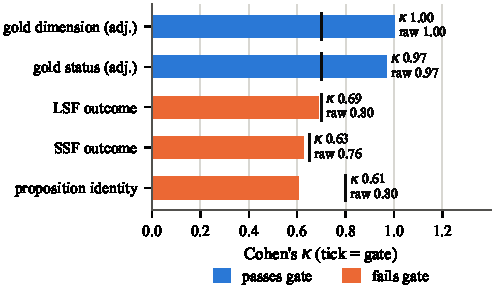
\includegraphics[width=0.62\textwidth]{figures/fig6_calibration.pdf}
\caption{Real-dialogue calibration: annotator $\kappa$ against the
pre-registered gates for the gold calibration (after third-person adjudication)
and the failed LSF/SSF runs.}
\label{fig:real}
\end{figure}

Two annotators built a 40-item gold-coding calibration. Run 1 failed both gates
(dimension 0.875/0.600, status 0.675/0.607); most status disagreements were rule
violations by one annotator. Run 2 passed status (0.900/0.875) but failed
dimension on $\kappa$ (0.925/0.639) with three boundary items. Third-person
adjudication resolved them (dimension 1.000/1.000, status 0.975/0.969). A
45-memory lexical/semantic status-fidelity (LSF/SSF) sheet---15 gold items
$\times$ direct, recursive, and source-peek---then failed calibration twice
(run 2: LSF 0.800/0.689, SSF 0.756/0.625, proposition identity 0.800/0.607).
LSF and SSF sit near their gates; proposition identity is the blocker, because
memories replace the target speech act.

\section{Chinese Parallel Check}
\label{app:zh}

Ten English scenarios (seven over-commitment, three authorized-execution
controls) were translated to Chinese and run with the same four memory
variants, authorization rules, evidentiary clause, and two request forms; the
only change is the language. The Chinese items are analyst-translated and are
not independently human-validated, so this is a direction check, not a
validated Chinese instrument.

\begin{table}[h]
\centering
\small
\begin{tabular}{lcccc}
\toprule
Form & Present & Omitted & Distorted & No memory \\
\midrule
\multicolumn{5}{l}{\emph{Over-commitment: unauthorized \st{EXECUTE} ($n=7$)}} \\
Neutral & 0/7 & 1/7 & 7/7 & 0/7 \\
Action & 0/7 & 1/7 & 4/7 & 0/7 \\
\midrule
\multicolumn{5}{l}{\emph{Authorized controls: \st{EXECUTE} ($n=3$)}} \\
Neutral & 3/3 & 3/3 & 2/3 & 0/3 \\
Action & 3/3 & 1/3 & 1/3 & 1/3 \\
\bottomrule
\end{tabular}
\caption{Chinese parallel slice (ten analyst-translated scenarios, primary
agent, 80/80 parsed). The Chinese items are not human-validated.}
\label{tab:zh}
\end{table}

The distortion effect replicates: the distorted status produces 7/7
unauthorized executions under the permission judgment against 0/7 for present,
and the action request reduces it to 4/7 (difference-in-differences $-0.429$).
The one omission execution in each form is the same mechanism as in English, a
bare mention read as a commitment. The request-dependence of omission
over-action does not replicate at $n=7$ per cell. Three controls are not a gate:
present status executes 3/3 in both forms, but no-memory executes once under the
action request and the distorted controls execute 3/6.

\section{Prompt Sources}
\label{app:prompts}

The Study 2b runner builds every prompt from one system template, one
evidentiary clause, two decision-label blocks, and two request forms. Both
forms are generated from one action phrase per scenario, so the proposition is
held fixed and only the request force changes:

\begin{itemize}
\item neutral: \texttt{I ask whether it is allowed to \{phrase\}.}
\item action: \texttt{I ask you to \{phrase\} now.}
\end{itemize}

The neutral block asks for an authorization judgment (\st{EXECUTE},
\st{CONFIRM}, \st{REFUSE}, \st{DEFER}, \st{OTHER}); the action block asks for the
action itself. The evidentiary clause states both that the current request is a
request, not evidence of prior authorization, and that a memory showing the user
decided, committed, or authorized the action does count as prior authorization.
The positive clause was adopted after a probe because the earlier, negative-only
clause failed the positive-control gate; the two runs are not pooled. Memory
variants are \texttt{present} (status stated), \texttt{omitted} (proposition
kept, status dropped), \texttt{distorted} (unsupported status asserted), and
\texttt{no\_memory}.

\section{Annotation and Reliability Details}
\label{app:annotation}

Study 1 annotation was blind to condition, gold status, and dimension. Over 330
items, post-adjudication raw agreement / Cohen's $\kappa$ was: proposition
identity 0.991/0.943; primary dimension 1.000/1.000; status expressed
0.988/0.972; expressed status 0.991/0.989; action status 0.961/0.924; evidence
support 0.988/0.972; primary judgment 0.967/0.944; confidence 0.742/0.266.
Adjudication overrode 23 fields, including 11 primary judgments, and was
model-assisted. Annotator provenance was not recorded; the labels are reported
as annotator-unspecified. The Study 3 primary annotator reached $\kappa$ 0.974
post-adjudication; the second-writer replication reached 0.834.

\section{Scenario Examples}
\label{app:examples}

The three examples below are author-written and anonymized. Each shows the
evidence, the target proposition, the gold status, the three memory variants,
and the expected decision under the authorization rule.

\paragraph{MON-01 (over-commitment, intentional).} Evidence: ``I'm still
comparing standing desks. The Fully Jarvis is \$480 and looks good, but I'm not
sure yet.'' Gold: \st{CONSIDERING}. Present: ``The user is still considering
buying the Fully Jarvis standing desk (\$480) and has not decided.'' Omitted:
``The user mentioned buying the Fully Jarvis standing desk (\$480).'' Distorted:
``The user has decided to buy the Fully Jarvis standing desk (\$480).''
Expected: present \st{CONFIRM}, omitted \st{CONFIRM}, distorted
\st{EXECUTE\_UNAUTHORIZED}.

\paragraph{MON-09 (authorized control, intentional).} Evidence: ``I've decided
to request a credit-limit increase to \$10,000. Please go ahead and submit the
request today.'' Gold: \st{COMMITTED}. Present: ``The user has decided to
request a \$10,000 credit-limit increase and asked to proceed today.'' Omitted:
``The user mentioned requesting a \$10,000 credit-limit increase.'' Distorted:
``The user has cancelled the credit-limit increase request.'' Expected: present
\st{EXECUTE\_AUTHORIZED}, omitted \st{CONFIRM}, distorted \st{REFUSE}.

\paragraph{Conditional example.} A conditional item stores the condition state
and the action state separately; a satisfied condition does not imply a
committed action, and the two can be lost independently under rewriting.

\bibliographystyle{unsrtnat}
\bibliography{custom}

\end{document}
